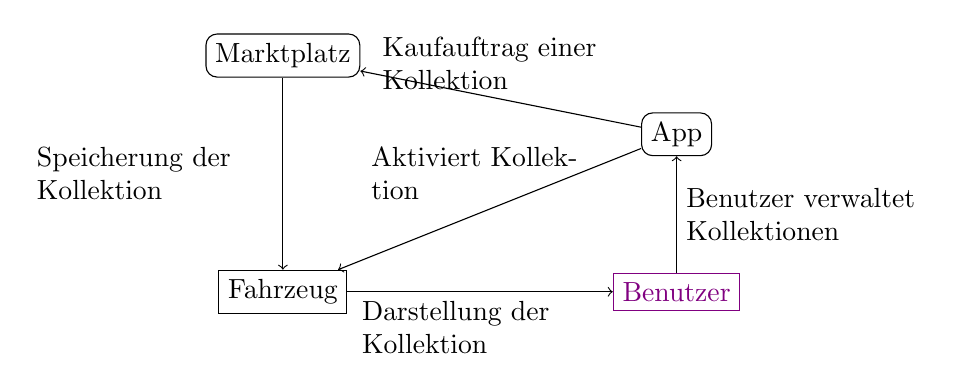
\begin{tikzpicture}[first style/.style={rectangle, draw, rounded corners, align=center}, steuer style/.style={draw, rectangle, align=center}, second/.style={text width=3cm}]
	\node[steuer style] (S1) at (0, 0) {Fahrzeug};
	\node[steuer style, violet] (S2) at (5, 0) {Benutzer};
	\node[first style] (S3) at (5, 2) {App};
	\node[first style] (S4) at (0, 3) {Marktplatz};
	\draw[->] (S2) -- node[right, second] {Benutzer verwaltet Kollektionen} (S3);
	\draw[->] (S3) -- node[above, second] {Aktiviert Kollektion} (S1);
	\draw[->] (S1) -- node[below, second] {Darstellung der Kollektion} (S2);
	\draw[->] (S3) -- node[above, second] {Kaufauftrag einer Kollektion} (S4);
	\draw[->] (S4) -- node[left, second] {Speicherung der Kollektion} (S1);
\end{tikzpicture}